\subsection{Bedarfserkennung von Software}\label{bedarfserkennung}
Im Rahmen der Bedarfserkennung steht die Beschreibung der eigenen Umgebung von Fahrzeugen im Mittelpunkt. Damit die Softwarehersteller den Bedarf von Fahrzeugen abdecken können, muss ihnen die Umgebung des Fahrzeugs zu dem Zeitpunkt der Bedarfserkennung bekannt sein. Um zu verstehen, wie ein Fahrzeug seine Umwelt eigens beschreiben kann, wird im Folgenden die Architektur eines autonomen Fahrzeugs vorgestellt und erläutert, welche Bestandteile dessen für die Bedarfserkennung relevant sind. 
\subsubsection{Relevante Systeme eines autonomen Fahrzeugs in der Bedarfserkennung}
Um die Suche nach Software zu erleichtern, benötigt die Suche auf dem Server gewisse Daten als Input. Damit die Situation, in welcher das Fahrzeug nicht selbstständig fahren kann, durch eine Software abgedeckt werden kann ist es wichtig eine Beschreibung der Umwelt des Autos zu dem Zeitpunkt der Bedarfserkennung zu erstellen. Durch die Fusion aufgenommener Kamera-, Ultraschall- und Radardaten kann die Umwelt beziehungsweise die Umgebung des Autos in einem Datenformat wie dem von der ASAM\footnote[1.]{https://www.asam.net/standards/detail/openscenario/} definierten Standard "OpenSCENARIO"\cite{b35} dargestellt werden. Dieser wird in Kapitel \ref{2.2} vorgestellt.\\
Im Rahmen der Suche nach möglicherweise nötiger Software spielt die Routen- und Bewegungsplanung des Autos eine große Rolle. Zum einen kann das Auto bei der Eingabe einer neuen Route diese nach Gegenden absuchen in denen oft neue Software benötigt wird. Es kann infolgedessen diese dem Fahrer bereits vor Fahrtbeginn vorschlagen und somit die Bequemlichkeit der Fahrt sicherstellen. Zum anderen soll das Auto  Muster im Fahrtenverlauf erkennen, um so bei der Erkennung eines Softwarebedarfs auf einer dieser Strecken eben diese Software zum Kauf vorzuschlagen.\\
Abbildung 1 zeigt die Architektur eines Autonomen Fahrzeugs nach Jeff Schneider. Sie verdeutlicht, welche Bestandteile ein Autonomes Fahrzeug besitzt um mit Hilfe dieser selbstständig zu Fahren. Die aufgenommenen \textit{Sensordaten} leiten Informationen an die \textit{Karten- \& Positionsverfolgung} weiter. Durch einen Merge (Zusammenführung) dieser Daten kann das Fahrzeug die eigene Umwelt \textit{wahrnehmen} und mit Hilfe der dynamischen Inhalte der Welt (zB. Geschwindigkeiten) \textit{Vorhersagen} für den Verkehr stellen. Als Bündel stellen sie die Bewegungsplanung dar.
\begin{figure}[H]
	\centering
	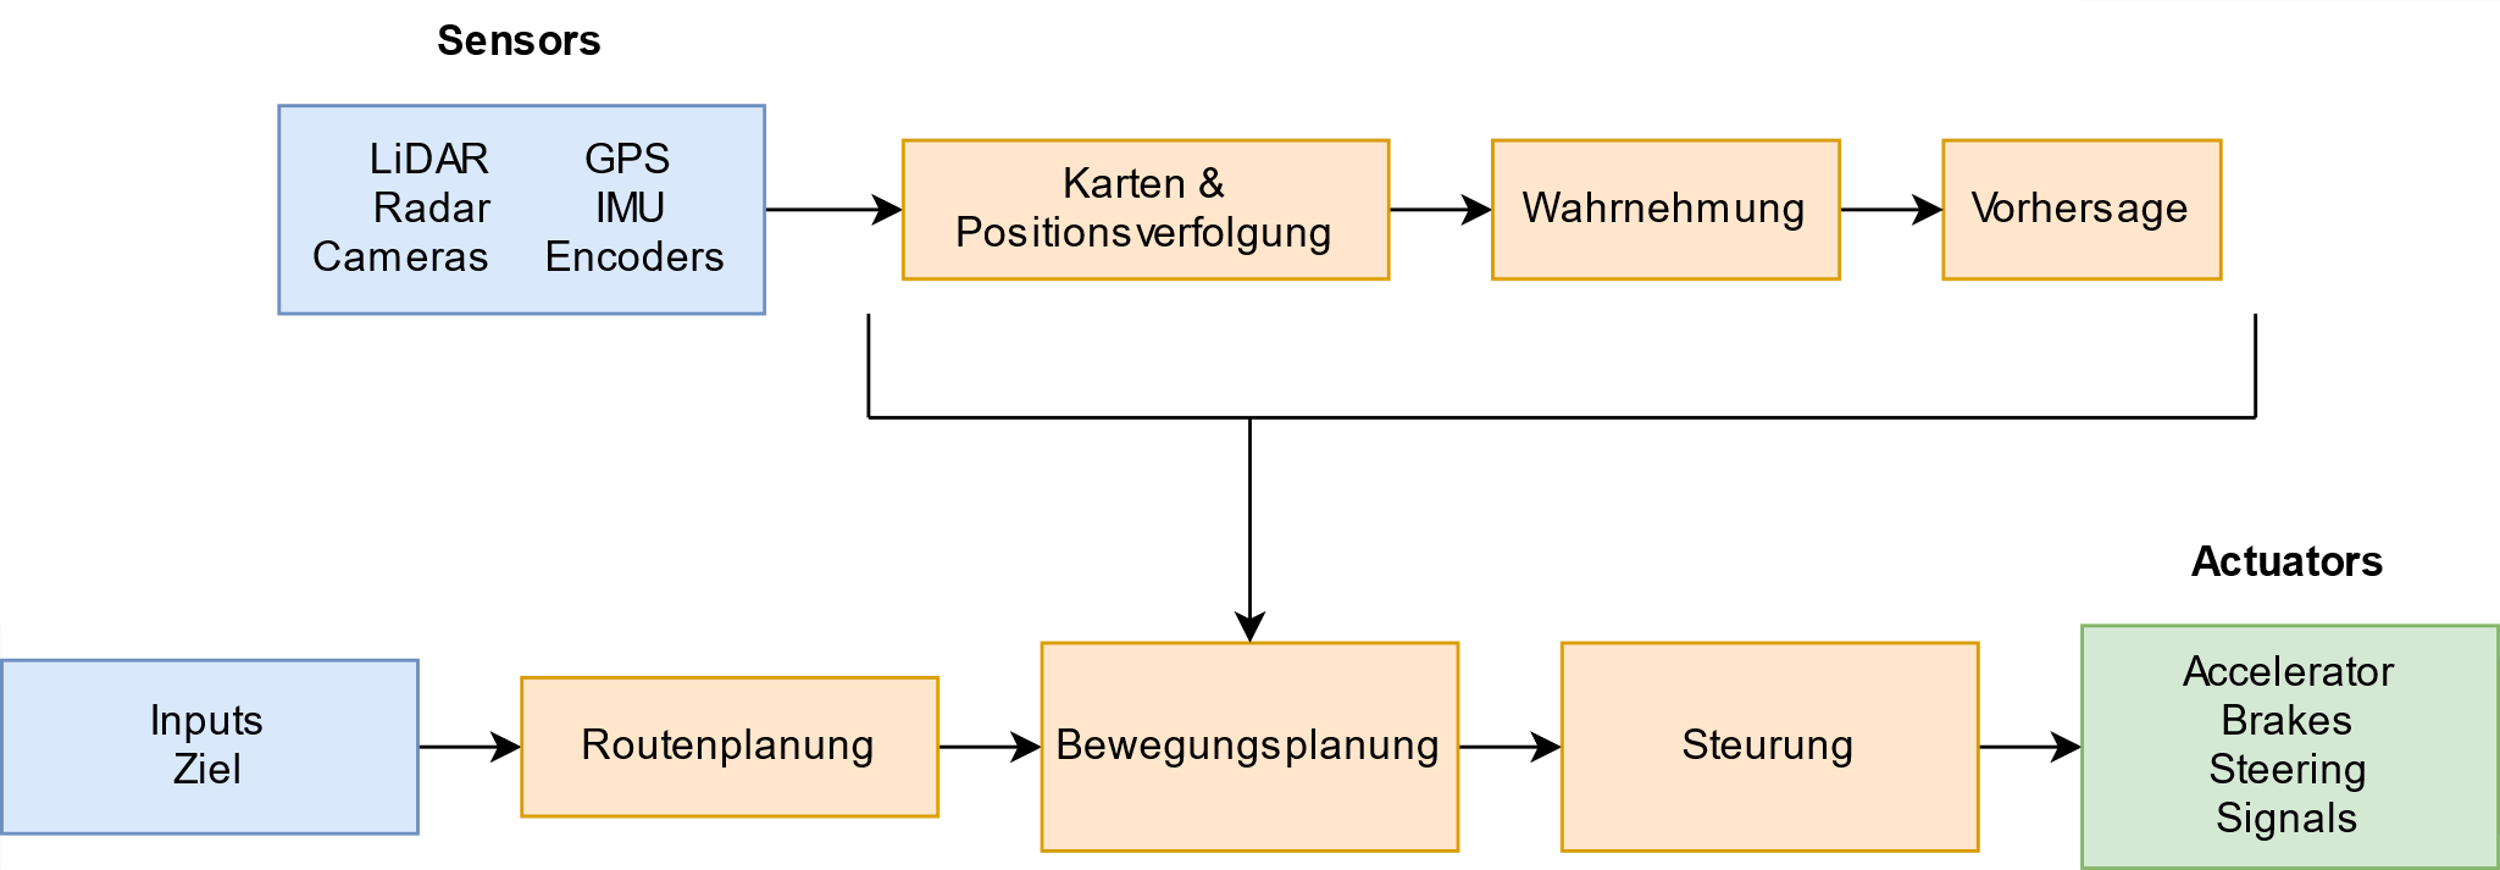
\includegraphics[width=0.95\textwidth]{../pictures/arichtecture_AV.png}
	\caption{Architektur AV nach Jeff Schneider (CMU) \cite{jschneider}}
\end{figure}
Der Fahrer gibt dem Auto initial ein \textit{Ziel}, mit Hilfe dessen das Fahrzeug die zu fahrende Route berechnet. Die Bewegungssteuerung gibt das Wahrgenommene und Vorhergesagte weiter an die Steuerung welche letztendlich entscheidet, was die einzelnen Aktuatoren machen.
Damit der Bedarf einer Softwarelücke festgestellt werden kann, müssen die Systembausteine "Sensoren", "Karten \& Positionsverfolgung", "Wahrnehmung" und "Vorhersage" angeknüpft werden um so herauszufinden \textbf{wann} das Fahrzeug nicht mehr selbstständig fahren kann. Wurde dieser Moment festgestellt, wird die Übergabe der Fahraufgabe initiiert und zeitgleich auch die Suche nach Software gestartet.\\
Neben den wichtigen Bausteinen der Bewegungsplanung kann auch anhand der Routenplanung von Fahrzeugen ein Softwarebedarf untersucht werden (Siehe \ref{2.3}). Zunächst wird eine Möglichkeit dargestellt, wie die Daten der Bewegungsplanung in einer geeigneten Form gespeichert und versendet werden können.
\subsubsection{Eine geeignete Kommunikationsgrundlage: OpenSCENARIO}\label{2.2}
Der Inhalt dieses Kapitels basiert auf Inhalten der Projektwebseiten des OpenSCENARIO Standards.\cite{b35}.\\
OpenSCENARIO ist ein XML-basiertes Dateiformat zur Beschreibung aller statischen \textit{(Gegenstände, Hindernisse, etc.)} und dynamischen\textit{(Geschwindigkeiten, Bewegungsrichtungen, etc.)} Inhalte der Umwelt eines Fahrzeugs. "Der primäre Anwendungsfall von OpenSCENARIO ist es komplexe, synchrone Manöver zu beschreiben, welche mehrere Entitäten wie Fahrzeuge, Fußgänger und andere Verkehrsteilnehmer betreffen."(Vgl. \cite[asam.net]{b35})\\

Abbildung 2 zeigt einen Ausschnitt einer OpenSCENARIO-Datei. Für ein Szenario ist immer das \textbf{Straßennetzwerk}\textit{ (RoadNetwork) }sowie die beinhalteten \textbf{Entitäten }\textit{(Entities)} festzulegen. Das eigentliche Szenario ist innerhalb eines \textbf{Storyboards }dargestellt und unterteilt sich in einzelne \textbf{Storys }\textit{(Siehe Abbilung 2)}. Alle zuvor definierten Entitäten erhalten eine initiale \textbf{Action}, welche das initiale Handeln der Entität festlegt (Siehe <Init>-Block).\\
Eine einzelne Story ist immer einer einzelnen Entität zuzuordnen. Eine Story wiederum ist in \textbf{"Acts"} aufgeteilt, welcher eine Sammlung an \textbf{"Sequenzes"} beinhalten kann. Jedes dieser Elemente kann mit einer \textbf{"Condition"} versehen werden. Wird die "Condition" (Bedingung) erfüllt, wird der jeweilige Story-/Act- oder Sequenz-Block ausgeführt.
\begin{figure}[H]
	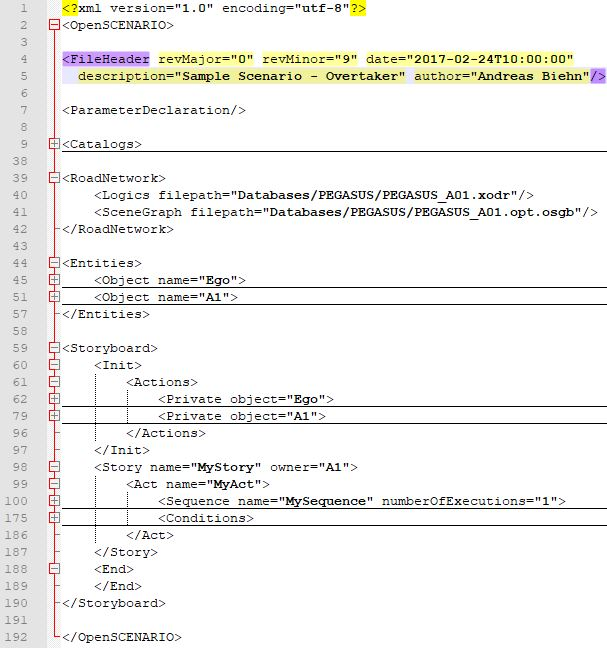
\includegraphics[width=\textwidth]{../pictures/openscenario.jpg}
	\caption{Ausschnitt einer OpenSENARIO Datei von Andreas Biehn\cite[(Downloads)]{b35}}
\end{figure}
OpenScenario ist aus mehreren Gründen gut geeignet um als Kommunikationsgrundlage zwischen Auto und Server zu fungieren. Zum einen handelt es sich dabei um eine Opensourcelösung, wodurch jeder Entwickler Weltweit selbstständig mit diesem Arbeiten kann. Zum anderen existiert wegen dem XML-basierten Dateiformat eine gute Lesbarkeit und Regelmäßigkeit Abfolge der Szenarien. Ein Szenario kann aufgrund dieser Regelmäßigkeit einfach und schnell erstellt werden. Der letzte und größte Vorteil von OpenScenario ist es, dass man ein Szenario in dem Opensource Simulator "Carla" abspielen kann.\\
Der im Folgenden vorgestellte Software-User-Pattern-Recognizer (SUPR) nutzt das OpenScenario-format zur Suche nach Software. Welche Suchvarianten es gibt und weitere Aufgaben des SUPR werden hier vorgestellt.

\subsubsection{Software-User-Pattern-Recognizer [SUPR] im Rahmen der Bedarfserkennung}\label{2.3}
Das in diesem Abschnitt vorgestellte Konzept des Software-User-Pattern-Recognizer (kurz: SUPR) ist ein eigens ausgearbeiteter Baustein, welcher die Bedarfserkennung für intelligente Fahrzeuge beschleunigen und vereinfachen soll. Die Aufgaben des SUPR lassen sich in Aspekte der Bedarfserkennung sowie der Bereitstellung aufteilen, weshalb der SUPR in Kapitel 3.3 wieder aufgegriffen wird.\\
Eine Aufgabe des SUPR im Rahmen der Bedarfserkennung ist es, auf Anfrage hin eine Suche nach passenden Softwarepaketen durchzuführen \textbf{(1.)}. Die zweite Aufgabe ist die regelmäßige Suche nach Software in der Umwelt/Region des Autos bzw. die Suche nach Softwarepaketen entlang zu Fahrender Strecken \textbf{(2.)}. Das Maß der Rechenleistung auf Seiten des Servers ist indes höher als auf dem Fahrzeug. Eine mögliche Gegenüberstellung von Rechenleistung und Sendeleistung des Servers und des Autos kann zu behebende Defizite der Architektur aufdecken - die Optimierung des Systems ist jedoch nicht Teil des Forschungsseminars.\\
Der Server, auf welchem die Suche stattfindet, benötigt zwei Datenbanken: die eine enthält sämtliche Softwarepakete für intelligente Fahrzeuge, die andere eine große Menge an OpenScenario Dateien, welche zusätzlich Fremdschlüsselverweise auf ein oder mehrere Softwarepakete bereitstellen. Nur wenn diese Bedingung erfüllt ist, kann eine Suche durchgeführt werden. 

\textbf{1. Gezielte Suchanfragen}\\
Gerät ein intelligentes Fahrzeug im Laufe seiner Fahrt in eine ihm unbekannte Situation, kann es diese mit Hilfe von OpenSCENARIO beschreiben. Das vom Auto erstellte Szenario wird an den Server geschickt, welcher dieses mit den auf der Datenbank liegenden Szenarien abgleicht. Ist die Suche abgeschlossen, wird eine Fallunterscheidung zwischen den folgenden Optionen getätigt:
\begin{itemize}
	\item[A] \textbf{Es wird \textbf{kein} passendes Softwarepaket gefunden}\\
	Entweder existiert zu dem übergebenen Szenario keine Software oder möglicherweise wurde die im Szenario dargestellte Situation noch nicht zu einer Software gemapped. Dies sollte von speziell hierfür angestellten Arbeitnehmern überprüft werden, um so Dopplungen in der Softwareentwicklung zu vermeiden. 
	\item[B] \textbf{Es werden (mehrere) passende Softwarepakete gefunden.}\\
	In diesem Fall gilt zu entschieden, welches Softwarepakete die besten Auswirkungen auf die Performance des Autos hat. 
	Hierzu ist das Heranziehen diverser Kennzahlen ratsam um somit die Performance der unterschiedliches Softwares untereinander zu vergleichen und eine fundierte Entscheidung treffen zu können. Eine beispielhafte Ausarbeitung dieser Entscheidungstreffung stellt Niklas Stelter in seiner Bachelorarbeit vor\cite{stelter}. Am Ende einer Suche soll entweder eine einzelne oder keine Software vorgeschlagen werden.
\end{itemize}
Neben der vom Fahrzeug ausgehenden Suche nach einer bestimmten Software, kann dieses auch Vorschläge für Software von einem Server erhalten, welcher dauerhaft die Umwelt intelligenter Fahrzeuge analysiert.

\textbf{2. Ortsbezogene Erkennung eines Softwarebedarfs}
Neben der Suche nach einer bestimmten Software soll der SUPR auch Suchen in der Heimatregion des Autos durchführen sowie auf zu Fahrenden Strecken. Diese Suchen basieren nicht auf OpenScenario-Dateien sondern auf Basis der Routenplanung\textbf{[A]} (Siehe Abbildung 1) und der Fahrtenhistorie des Fahrzeugs\textbf{[B]}.\\

\textbf{\textit{A: Suche auf Basis der Routenplanung}}\\
Wird vom Fahrer eine nicht oft oder noch gar nicht zurückgelegte Strecke vorgegeben, so soll der SUPR entlang der zu fahrenden Strecke häufig auftretenden Softwarebedarf identifizieren und dem Fahrer vor oder kurz nach Antritt der Reise diese Softwarevorschlagen. Daraus ergibt sich die Anforderung, zu jedem sich in der Datenbank befindlichen OpenScenario auch die geographische Position der Bedarfsentdeckung zu speichern. In Abbildung 3 ist folgende Situation dargestellt: Unser Auto hat als Ziel im Navigationssystem "Braunschweig" erhalten und befindet sich aktuell auf der A2. Die roten Boxen stellen den möglichen Bereich dar, in welchem der Server die Umweltanalyse betreibt. Wird eine Software entdeckt, überprüft das System die Relevanz für das eigene Fahrzeug und schlägt sie je nach dem vor oder nicht.
\begin{figure}[H]
	\centering
	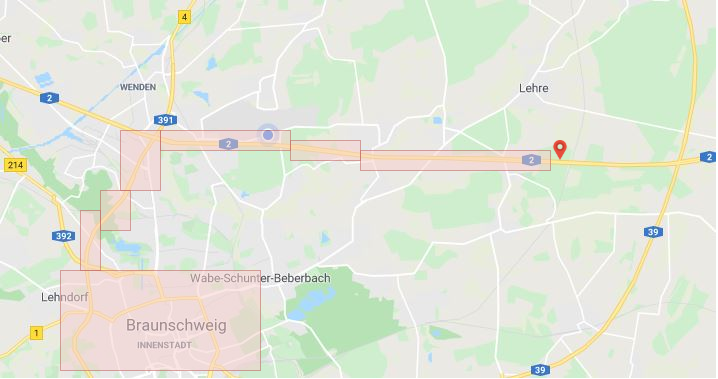
\includegraphics[width=0.95\textwidth]{../pictures/umweltanalyse.png}
	\caption{Umweltanalyse}
\end{figure}

\textit{\textbf{B: Suche auf Basis der Fahrtenhistorie}}\\
Hierbei werden Muster in den zurückgelegten Strecken des Fahrers gesucht, um so dessen meist gefahrene Strecken zu identifizieren. Das Auto soll abschätzen können, wann der Fahrer welche Strecke zurücklegen wird. Vor dem jeweiligen Fahrtantritt soll die Suche nach Software identisch zu Variante A durchgeführt worden sein. Der Unterschied ist, dass die Suche hierbei selbstständig erfolgen soll, was ein besseres Nutzungserlebnis für den Fahrer schafft.\\

Ist die Suche \textit{(egal ob gezielte Suche oder Umweltanaylyse)} abgeschlossen, kann die Software dem Fahrer zum Kauf vorgeschlagen und bei Bestätigung für das Auto bereitgestellt werden. Das nächste Kapitel verdeutlicht den Umfang der Bereitstellung.